\subsection*{Hypothesis 6}

\textbf{H0 (Null Hypothesis):} There is no correlation between the number of books published for a category (or publisher) and the review score.\\
All data cleaning and transformation steps were executed using MongoDB's aggregation pipeline to ensure efficient and rapid computation.
Specifically, data cleaning involved the use of the \textit{\$match} operator, while data transformation steps were carried out with
the \textit{\$group} operator, utilizing the \textit{\$avg} operation. Finally, the \textit{\$project} operator was applied to select
the relevant fields. To reduce bias, we excluded categories with fewer than 50 books and publishers with fewer than 20 books.
The results are presented in Table \ref{tab:h6_correlations}.\\
\textbf{Conclusion:} The hypotheses are rejected as the metrics reveal no significant correlation between the number of books published
for a category (or publisher) and the review score in both cases.

\begin{table}[H]
    \footnotesize
    \centering
    \caption{Correlation Values and P-values for Categories and Publishers}
    \begin{tabular}{|c|c|c|}
        \hline
        \textbf{Variable} & \textbf{Correlation Value} & \textbf{P-value} \\
        \hline
        Category          & -0.0806                    & 0.558            \\
        \hline
        Publisher         & -0.0673                    & 0.151            \\
        \hline
    \end{tabular}
    \label{tab:h6_correlations}
\end{table}

\textbf{Curiosity:}
We executed two complex MongoDB queries to answer two intriguing questions:

\begin{itemize}[leftmargin=*, noitemsep]
    \item \textbf{Which are the best publishers?} (i.e., those capable of achieving average scores above 4.5 in multiple categories)
    \item \textbf{In which categories are the best publishers focused?}
\end{itemize}

The results of these queries are presented in Figure \ref{fig:h6_which_best} and Figure \ref{fig:h6_where_best}.

\begin{figure}[H]
    \centering
    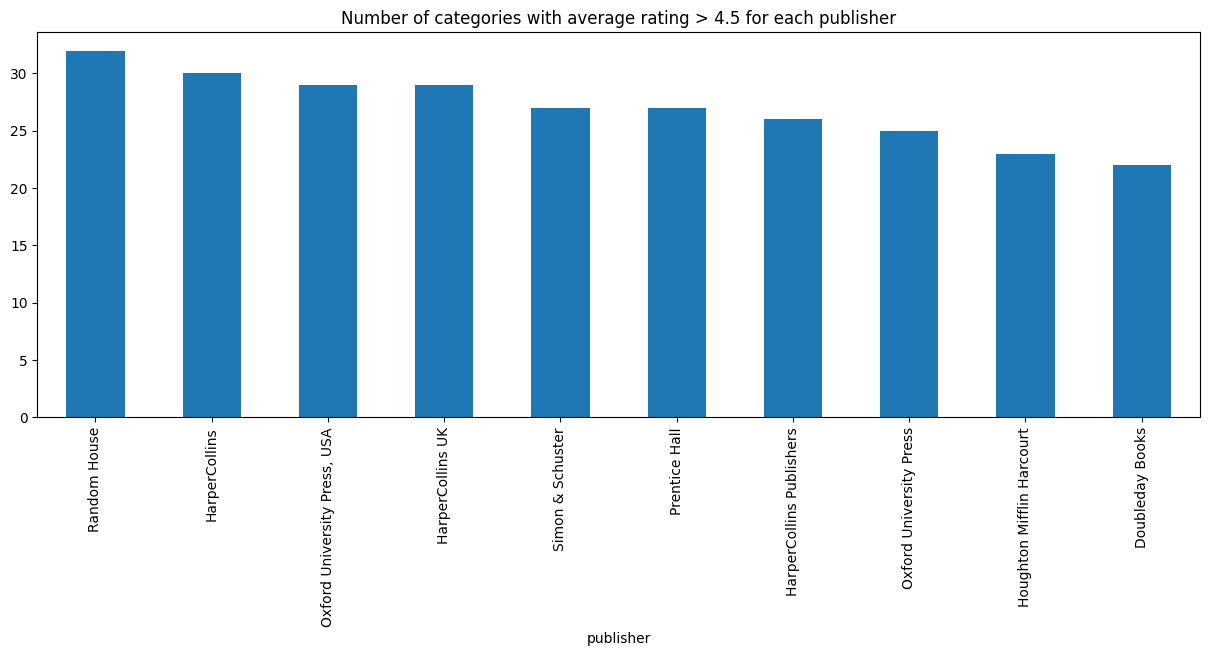
\includegraphics[width=0.4\textwidth]{./figures/h6_which_best.png}
    \caption{Identifying the Best Publishers}
    \label{fig:h6_which_best}
\end{figure}

\begin{figure}[H]
    \centering
    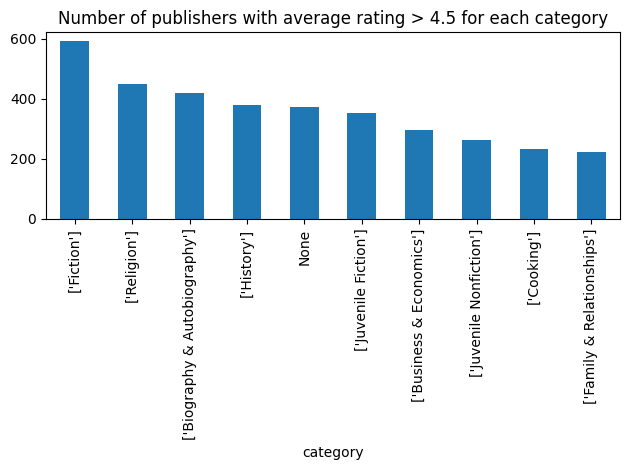
\includegraphics[width=0.4\textwidth]{./figures/h6_where_best.png}
    \caption{Categories Favored by the Best Publishers}
    \label{fig:h6_where_best}
\end{figure}
